\documentclass{amsart} 
\usepackage{graphicx}
\graphicspath{{./}}
\usepackage[fontsize=14pt]{scrextend}
\usepackage{hyperref}
\usepackage{csvsimple}
\usepackage{epigraph}
\title{Single Human Race Scientific Attribution}
\author{Zulfikar Moinuddin Ahmed}
\date{\today}
\begin{document}
\maketitle

\section{Introduction}
We live in an age that has not absorbed one of the most important pieces of knowledge regarding who we are.  In the distant future, this will become children's kindergarden knowledge, but today it is not.  Science had known for a very long time that 'races' are political fiction and not biological reality.  I will confess that I did not know this myself, because when I was in high school, this was simply not known. There are so many confusions about these because racial propaganda and racial strife has been part of our history as well.  For these reasons, one has to be extremely overwhelming in compelling material when attempting to change the beliefs and opinions of 7.8 billion people.

In this note our goal will be to pay careful attention to a great peer-reviewed article by a multi-ethnic team of reputable scientists in one of the top science journals in the world, Science, in 2008.  It is the article \cite{Li08}.

\section{Our Descent from a single meta-tribe 75,000 years ago from East Africa}

Let us go back to \cite{Li08}.  In the abstract the authors write, 

"The relationship between haplotype heterozygosity and geography was consistent with the hypothesis of a serial founder effect with a single origin in sub-Saharan Africa."  

This is the most important issue to deduce a single human race.  This translates to much simpler lanuage of, "All human beings originate from Sub-Saharan Africa according to the measure of 'haplotype heterozygosity'."  Combine this with another peer-reviewed reputable scientific article \cite{SM} which details what else is known to determine the time of spreading out of all non-African populations, and we can understand that it was 75,000 years ago from a meta-tribe in East Africa.

\section{What Can Race Mean?}

What exactly is 'Race'?  Can you really call the descendents of a single tribe in East Africa multiple races even if 75,000 years pass?  For six million years before this Homo Sapiens evolved, and we were geographically concentrated.  Now purely logically it makes little rational sense to consider descendents of a single tribe to be different races.  That simply jars the ordinary human understanding of the sense of the word.  Obviously, if we are distant fourth cousins, we are not a different race.  We might enjoy each others' company or we might detest each other's taste and lifestyle but we cannot be a different race.  Similarly, this paper clearly tells us that regardless of their other findings, the single human race hypothesis is unchallenged.

\section{The 7 class results differentiating people}

I have seen some articles suggesting that the moment some clustering on genome is able to distinguish continental groups or ancestry, we should confirm Carl Linnaeus taxonomy into 5 races.  That is not substantive at all, since regardless of our technical ability to distinguish groups by some genetic differentiation, we are descendents of the same meta-tribe in East Africa (for non-Africans) and therefore the same race.

One might object and say, well there are group differences in genome, so what is the problem in considering them different races?  The total variation is minor genetically with maximum difference of 3-7\% of genome for any two groups, so what is the fundamental purpose.  We shared six million years of evolution, so our genetic similarity is overwhelming.  I find a rather conspicuous absence in various anti-politically correct accounts of the elephant in the room, which is that we know from the same analysis where 'races' are apparently found the strong support of single origin and dispersion around 75,000 years ago from East Africa.  {\em That} is the elephant in the room, not that afterward there is detectability in genes of differences that seem to confirm Linnaeus taxonomy.  We did not just all evolve in different places.  Homo Sapiens evolved millions of years ago before 75,000kya for dispersion. 

\section{The Rosenberg et. 2002 Paper}

Rosenberg et. al. (2002) \cite{Ros02} included an early use clustering to detect classes in genome of the world.  The following is their result of automatic clustering from $K=1,\dots, 6$.

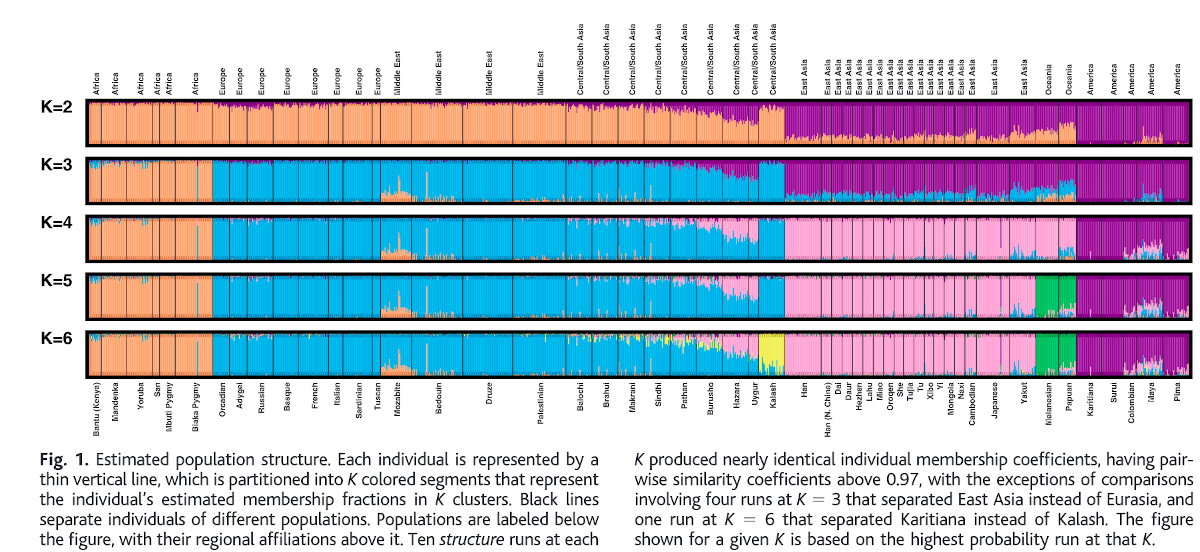
\includegraphics[scale=0.3]{clusterpop.png}

In none of these clusters do you find a separation of French from Palestinians or Baluchis.  So at least in a natural attempt, there was no simple differentiation of white Europeans from most of the Middle East.  This is extremely important to note, because one of the most trenchant parties today are European and American far right who are obsessed with 'white superiority' and think that people claiming single race are not supported by hard science.  If you are white-oriented, you will not find deep scientific solace for the meaning you want to put for the Crusades in this paper.

Now going back to the other parts of the paper, let me quote: 

"The average proportion of genetic difference between populations only slightly exceeds that between unrelated individuals of the same population.  That is, the within-group component of the genetic variation is estimated here at 93 to 95\%, accounts for most of the genetic diversity."

This is literally sufficient to make the claim that the human race is a single race.  From the genetic point of view, the rest of the variation is window dressing.  

In particular, people who make enormous efforts to find various types of superiority in the population will be sorely disappointed if they think that genes will grant them their wish.  Every functional of genes will find rough correspondence in other populations.  I am not impressed by the logic of the far right here who pretend that they have some secret access to har hitting scientific certainty while it is political correctness that is disallowing science to examine the real truth of racial superiority.  Rather, the human race is a single race, and the issues of group differences are difficult {\em precisely because we share a great percentage of genome across the globe}.  In this matter, politics had always appealed to the pride and gullibility of masses because tribal tendencies are universal genetic features of human race as well.

\section{Disclosure}

I have great personal interest in ensuring that the Human Race is a Single Race.  A lot of other things I don depend on it.  I am not about to let all sorts of fluffcakes bamboozle people with sloppy interpretations of scientific papers.


\begin{thebibliography}{CCC}
\bibitem{Li08}{ Li et. al., "Worldwide Human RelationshipsInferred from Genome-WidePatterns of Variation", Science, 319, 22  Feb 2008,1100--1104}
\bibitem{Ros02}{ Rosenberg et. al., "Genetic Structureof Human Populations", Science, 298, 2381--2384}
\end{thebibliography}

\end{document}